\subsection*{Equazione di Schroedinger per gli stati stazionari}

Ora, come si fa a prevedere l'andamento dell'equazione d'onda nel tempo e nello spazio?


Sia $\psi(\vec x, t) = \varphi(\vec c)F(t)$. Allora risulta
\[
    \psi = \varphi (\vec x) e^{\frac{-i}{\hslash}Et}F(0)
\]
e
\[
    |\psi|^2 = |\varphi(\vec x) F(0)|^2
\]
che non dipende dal tempo! Solo dalla posizione.

Risulta molto utile trovare le $\varphi$ tali che:
\[
    \H \varphi = E \varphi
\]
ovvero un problema di calcolo degli autovalori nello spazio delle funzioni.
\subsubsection*{Caso I 1D}
Ci si pone nella condizione in cui è presente solo una buca di potenziale nullo larga $a$ contornata da pareti a potenziale infinito:

\begin{figure}[h]
\centering
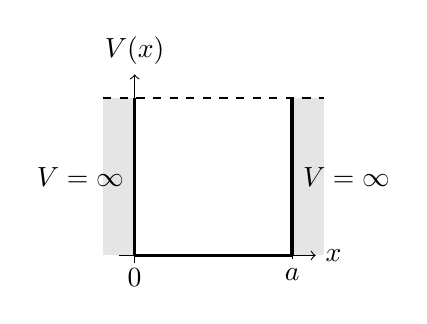
\begin{tikzpicture}[scale=2]
    \fill[gray!20] (-0.2,0) rectangle (0,1);
    \fill[gray!20] (1,0) rectangle (1.2,1);
    \draw[thick] (0,0) -- (1,0);
    \draw (0,0) -- (0,-0.02) node[below] {$0$};
    \draw (1,0) -- (1,-0.02) node[below] {$a$};
    \draw[dashed] (-0.2,1) -- (1.2,1) node[right] {};
    \draw[->] (-0.1,0) -- (1.15,0) node[right] {$x$};
    \draw[->] (0,-0.05) -- (0,1.15) node[above] {$V(x)$};
    \draw[very thick] (0,0) -- (0,1) node[midway,left] {$V=\infty$};
    \draw[very thick] (1,0) -- (1,1) node[midway,right] {$V=\infty$};
\end{tikzpicture}
\end{figure}

Si cercano le $\varphi : \H\varphi = E\vphi$. Nel caso 1D risulta inoltre che $\Lap = \sderiv{}$
\[
    \begin{cases}
        \H\vphi = E \vphi \\ 
        \vphi(0) = \vphi(a) = 0
    \end{cases}
\]
si pone $k^2 = \frac{2mE}{\hslash^2}>0$
\[
    \begin{cases}
        \vphi'' + k^2\vphi = 0\\
        \vphi(0) = \vphi(a) = 0
    \end{cases}
    \ \implies\ \ \vphi = A\cos(kx) + B\sin(kx),\ \ A = 0, kn = n\pi
\]
al ché si possono definire
\[
    \vphi_n(x) = B/sin(\frac{n\pi x}{a}),\ \ E_n = \frac{\hslash^2 n^2 \pi^2}{2 a^2 m}
\]

Queste sono tutte le armoniche, con energia $\propto n^2$. Ponendo poi $||\vphi_n||^2 = 1$ risulta, per ogni $n$, $B = \sqrt(\frac{2}{a})$ (ricavare per esercizio). Inoltre, dato che sono tutte soluzioni dell'equazione degli autovalori, tutte le $\vphi_n$ possono essere composte in una $\Phi$ pesate in modo che $||\Phi||^2 = 1$

Se invece si ha $\frac{2mE}{\hslash^2}<0$ risulta che non esistono soluzioni consistenti, in quanto gli esponenziali divergerebbero in tutte le direzioni.

\begin{figure}[h]
\centering
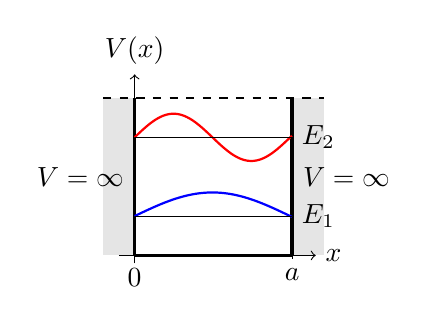
\begin{tikzpicture}[scale=2]
    \fill[gray!20] (-0.2,0) rectangle (0,1);
    \fill[gray!20] (1,0) rectangle (1.2,1);
    \draw[thick] (0,0) -- (1,0);
    \draw (0,0) -- (0,-0.02) node[below] {$0$};
    \draw (1,0) -- (1,-0.02) node[below] {$a$};
    \draw[dashed] (-0.2,1) -- (1.2,1) node[right] {};
    \draw[->] (-0.1,0) -- (1.15,0) node[right] {$x$};
    \draw[->] (0,-0.05) -- (0,1.15) node[above] {$V(x)$};
    \draw[very thick] (0,0) -- (0,1) node[midway,left] {$V=\infty$};
    \draw[very thick] (1,0) -- (1,1) node[midway,right] {$V=\infty$};
    
    % First sine at 1/4 height
    \draw[blue, thick] plot[domain=0:1, samples=100] (\x, {0.25 + 0.15*sin(pi*\x*58)});
    \draw[thin] (0,0.25) -- (1,0.25) node[right] {$E_1$};
    
    % Second sine (double frequency) at 3/4 height
    \draw[red, thick] plot[domain=0:1, samples=100] (\x, {0.75 + 0.15*sin(pi*\x*116)});
    \draw[thin] (0,0.75) -- (1,0.75) node[right] {$E_2$};
\end{tikzpicture}
\end{figure}

\subsection*{Particella libera e spettro continuo (1D)}
Come prima, si parte dell'equazione agli autovalori, però si ha che la buca di potenziale è infinitamente estesa (tutto R):
\[
    E< 0\ \implies\ \vphi'' - k^2\vphi = 0\ \implies\ \vphi = Ae^{-kx}+Be^{kx}\]\[
    E> 0\ \implies\ \vphi'' + k^2\vphi = 0\ \implies\ \vphi = Ae^{-ikx}+Be^{ikx}
\]
Tuttavia queste sono soluzioni 'improprie', in quanto in entrambi i casi non sono mai normalizzabili (addirittura divergono quelle della prima riga). Proviamo però con i pacchetti d'onda, considerando le onde monocromatiche $\vphi_k = \frac{1}{\sqrt{1\pi}}e^{ikx}$

\subsubsection*{Dinamica quantistica della particella libera}
Assemblando i passaggi precedenti:
\[
    \psi_k = \vphi_ke^{-\frac{i}{\hslash}E_kt} = \frac{1}{s\sqrt{2\pi}} e^{ikx -\frac{i}{\hslash}E_kt}
\]

Ora, i prossimi passaggi sono fare la trasformata dell'antitrasformata di Fourier di una distribuzione generica. Salta fuori la Funzione di Green \index{funzione di Green}, e il fatto che la densità di probabilità cambia nel tempo in funzione di TUTTI i possibili cammini da un punto della distribuzione iniziale al punto considerato. SI VEDANO GLI APPUNTI DER PROF 1d Problems infinite well pag 13

Risulta infine  
\[
    \psi(x,t) = \int_{-\infty}^{+\infty}\mathcal{G}(x-x',t)\psi(x',0)dx'
\]

\subsubsection*{Un caso particolare: wave packet spreading}
\[
    \psi(x,t) = \frac{\sqrt a}{(2\pi)^{3/4}}\rint e^{-\frac{a^2}{4}(k-k0)^2 + ikx - it\frac{\hslash k^2}{2m}}dk
\]
(tanti conti) Risulta:
\[
    \psi(x,t) \propto \exp(-\frac{2a^2(x-\hslash k_0t/m)}{a^4+4\hslash^2t^2/m^2})
\]
e quel che risalta è che questa gaussiana si muove nel tempo con velocità $v = \hslash k_0/m = \frac{P_0}{m}$ e varianza $\sigma = \sqrt{\frac{a^2}{4} + \frac{\hslash^2t^2}{4m^2a^2}}$. Siccome la varianza dipende dal tempo succede che, attendendo abbastanza tempo, una particella inizialmente localizzata si troverebbe ovunque con la stessa densità di probabilità!